\documentclass[11pt,letterpaper]{article}
\usepackage[margin=1in]{geometry}
\usepackage{amsmath,amssymb,amsfonts,bm,mathtools}
\usepackage{graphicx}
\usepackage{booktabs}
\usepackage[T1]{fontenc}
\usepackage{lmodern}
\usepackage{xcolor}
\usepackage[colorlinks=true,linkcolor=blue!60!black,citecolor=blue!60!black,urlcolor=blue!60!black]{hyperref}
\graphicspath{{../figures/}}

\newcommand{\vect}[1]{\mathbf{#1}}
\newcommand{\Ev}{\vect{E}}
\newcommand{\Hv}{\vect{H}}
\newcommand{\Jv}{\vect{J}}
\newcommand{\Mv}{\vect{M}}
\newcommand{\Nv}{\vect{N}}
\newcommand{\xv}{\vect{x}}
\newcommand{\kv}{\vect{k}}
\newcommand{\pv}{\vect{p}}
\newcommand{\mv}{\vect{m}}
\newcommand{\kp}{\kv_{\parallel}}
\newcommand{\xp}{\xv_{\parallel}}
\newcommand{\khat}{\hat{\kv}}
\newcommand{\rhat}{\hat{\vect{r}}}
\newcommand{\qhat}{\hat{\vect{q}}}
\newcommand{\nhat}{\hat{\vect{n}}}
\newcommand{\xhat}{\hat{\vect{x}}}
\newcommand{\yhat}{\hat{\vect{y}}}
\newcommand{\zhat}{\hat{\vect{z}}}
\newcommand{\ep}{\hat{\vect{e}}_p}
\newcommand{\dkk}{\,{\rm d}^2\kp}
\newcommand{\dO}{\,{\rm d}\Omega}
\newcommand{\II}{\mathbb{I}}
\renewcommand{\Re}{\operatorname{Re}}
\renewcommand{\Im}{\operatorname{Im}}
\newcommand{\Si}{\operatorname{Si}}
\newcommand{\code}[1]{\texttt{\small #1}}
\newcommand{\numcheck}[1]{\hfill{\small\color{green!40!black}[\,numerical check: #1\,]}}

\title{Derivations and numerical checks for optimal focusing\\[4pt]
\large Companion notes to Secs.~3.1--3.2 of ``Fundamental limits in photonics and electromagnetics: a tutorial''}
\author{Owen D. Miller}
\date{Draft, \today}

\begin{document}
\maketitle

\begin{abstract}
These notes collect the derivations behind the free-space focusing results (tutorial Sec.~3.1) and the complex-media focusing results (Sec.~3.2) of the tutorial by Miller and Monticone, at a level of detail that would be out of place in a tutorial of that breadth. Every closed-form result is checked numerically by a script in the accompanying repository. Each check is independent of the derivation it tests, e.g.\ brute-force quadrature with explicit polarization vectors, or a full multiple-scattering model. The achieved agreement is quoted in green alongside each result. Several results here are new relative to the tutorial text: closed forms for the full (anisotropic) focal-plane fields, the exact energy penalties for super-oscillatory spots, a closed form for the three-dimensional space-time focus, and explicit symmetry conditions for the point-dipole media used to test Sec.~3.2.
\end{abstract}

\tableofcontents

%=============================================================================
\section{Conventions}
%=============================================================================
Fields are complex amplitudes with time dependence $e^{-i\omega t}$, the time-averaged Poynting vector is $\tfrac12\Re(\Ev\times\Hv^*)$, and $k=\omega/c$. The electric energy density at a point is $U=\tfrac14\varepsilon_0|\Ev|^2$, as in the tutorial. The numerical codes use natural units $\varepsilon_0=\mu_0=c=Z_0=1$ and report dimensionless ratios such as $(2\pi c/k^2)\,\varepsilon_0|\Ev(0)|^2/P$.

Spherical Bessel functions are denoted $j_\ell$, cylindrical ones $J_n$, and $\Si(u)=\int_0^u \sin t/t\,{\rm d}t$. Two integral identities are used repeatedly:
\begin{align}
    \int_{-\pi}^{\pi} e^{iu\cos\varphi}\cos(n\varphi)\,{\rm d}\varphi &= 2\pi i^n J_n(u), \qquad \int_{-\pi}^{\pi} e^{iu\cos\varphi}\sin(n\varphi)\,{\rm d}\varphi = 0, \label{eq:JA}\\
    \int_0^1 x^{\nu+1}(1-x^2)^{\mu} J_\nu(ax)\,{\rm d}x &= 2^{\mu}\Gamma(\mu+1)\,a^{-\mu-1}J_{\nu+\mu+1}(a) \qquad(\text{Sonine}), \label{eq:Sonine}
\end{align}
the first being the Jacobi--Anger (``Hansen--Bessel'') identity, and the second Sonine's first finite integral ($\Re\nu>-1$, $\Re\mu>-1$). With $j_\ell(a)=\sqrt{\pi/(2a)}\,J_{\ell+1/2}(a)$, the special cases needed below are
\begin{align}
    \int_0^1 \frac{\beta J_0(a\beta)}{\sqrt{1-\beta^2}}{\rm d}\beta &= j_0(a), &
    \int_0^1 \beta\sqrt{1-\beta^2}\,J_0(a\beta){\rm d}\beta &= \frac{j_1(a)}{a}, \nonumber\\
    \int_0^1 \frac{\beta^3 J_2(a\beta)}{\sqrt{1-\beta^2}}{\rm d}\beta &= j_2(a), &
    \int_0^1 \beta^2\sqrt{1-\beta^2}\,J_1(a\beta){\rm d}\beta &= \frac{j_2(a)}{a}, \label{eq:SonineCases}
\end{align}
together with the elementary results $\int_0^s \beta J_0(a\beta){\rm d}\beta = sJ_1(as)/a$, $\int_0^s\beta^2J_1(a\beta){\rm d}\beta=s^2J_2(as)/a$, and $\int_0^s\beta^3J_2(a\beta){\rm d}\beta=s^3J_3(as)/a$ (all from $\tfrac{{\rm d}}{{\rm d}x}[x^{n}J_n(x)]=x^nJ_{n-1}(x)$), and $\int_0^s\beta^3J_0(a\beta){\rm d}\beta = s^3J_1(as)/a-2s^2J_2(as)/a^2$.

\paragraph{The extremal-eigenvalue lemma.} Every bound in these notes is an instance of the following. For a linear functional $f(c)=\langle v,c\rangle$ and a positive weight $g$,
\begin{align}
    \frac{|\langle v,c\rangle|^2}{\langle c, g\,c\rangle} \le \langle v, g^{-1} v\rangle, \qquad \text{with equality iff } c\propto g^{-1}v,
    \label{eq:CS}
\end{align}
by the Cauchy--Schwarz inequality applied to $g^{1/2}c$ and $g^{-1/2}v$. Equivalently, the quadratic form $c^\dagger(v v^\dagger)c$ is rank one, so its Rayleigh quotient is maximized by its only nonzero eigenvector.

%=============================================================================
\section{Focusing from a cone of plane waves (tutorial Sec.~3.1.2)}
%=============================================================================
\subsection{Plane-wave expansion and power}
A field produced by sources in $z<0$ and observed in a region free of sources is a superposition of propagating plane waves (evanescent components are excluded, as they are absent at far-field distances from the sources):
\begin{align}
    \Ev(\xv) = \sum_{p}\int \dkk\, c_p(\kp)\,\ep(\kp)\,e^{i\kv\cdot\xv}, \qquad
    \Hv(\xv) = \frac{1}{Z_0}\sum_{p}\int \dkk\, c_p(\kp)\,\khat\times\ep(\kp)\,e^{i\kv\cdot\xv},
    \label{eq:PW}
\end{align}
with $\kv=\kp+k_z\zhat$, $k_z=\sqrt{k^2-|\kp|^2}\ge0$, and $(\hat{\vect e}_1,\hat{\vect e}_2,\khat)$ a right-handed orthonormal triad. Numerical aperture $\sin\theta$ restricts $|\kp|\le k\sin\theta$. The $z$-directed power through a plane is
\begin{align}
    P &= \frac12\Re\int(\Ev\times\Hv^*)\cdot\zhat\,{\rm d}x\,{\rm d}y
    = \frac{(2\pi)^2}{2Z_0}\Re\sum_{p,p'}\int\dkk\, c_p c_{p'}^*\big[\ep\times(\khat\times\hat{\vect e}_{p'}^*)\big]\cdot\zhat \nonumber\\
    &= \frac{2\pi^2}{Z_0}\sum_p\int\dkk\,\frac{k_z}{k}|c_p(\kp)|^2,
    \label{eq:Power}
\end{align}
where the spatial integral produced $(2\pi)^2\delta(\kp-\kp')$ and $\ep\times(\khat\times\hat{\vect e}_{p'}^*)=\khat(\ep\cdot\hat{\vect e}_{p'}^*)-\hat{\vect e}_{p'}^*(\ep\cdot\khat)=\khat\,\delta_{pp'}$.
\numcheck{\code{power\_normalization\_check.py}: direct Poynting integration of FFT-synthesized fields with random complex spectra in both polarizations, relative error $\le7\times10^{-16}$}

\subsection{Optimal coefficients and the focal matrix}
The field at the focus in a (possibly complex) polarization $\qhat$ is $\qhat^*\cdot\Ev(0)=\sum_p\int\dkk\,c_p\,(\qhat^*\cdot\ep)$. We consider two normalizations,
\begin{align}
    \text{power:}\quad \frac{2\pi^2}{Z_0}\sum_p\int\dkk\,\frac{k_z}{k}|c_p|^2 = P, \qquad\qquad
    \text{amplitude:}\quad \frac{2\pi^2}{Z_0}\sum_p\int\dkk\,|c_p|^2 \equiv P_{\rm amp},
\end{align}
i.e.\ weights $g=k_z/k$ and $g=1$ in \eqref{eq:CS}. The optimal coefficients are $c_p\propto g^{-1}(\qhat^*\cdot\ep)^*$, i.e.\ $c_p^{\rm (opt)}\propto(k/k_z)(\qhat^*\cdot\ep)^*$ for power normalization, which is the tutorial's $\alpha_p^{\rm (opt)}\propto\sqrt{k/k_z}(\qhat^*\cdot\ep)^*$ written for $\alpha_p=\sqrt{k_z/k}\,c_p$. The maximum is
\begin{align}
    \max\frac{\varepsilon_0|\qhat^*\cdot\Ev(0)|^2}{P} &= \frac{\varepsilon_0 Z_0}{2\pi^2}\sum_p\int\dkk\,\frac{k}{k_z}|\qhat^*\cdot\ep|^2
    = \frac{1}{2\pi^2c}\,\qhat^\dagger\mathsf{M}\,\qhat, \nonumber\\
    \mathsf{M}&=\int\dkk\,\frac{k}{k_z}\big(\II-\khat\khat^{\rm T}\big),
    \label{eq:Mmatrix}
\end{align}
using the completeness relation $\sum_p\ep\ep^\dagger=\II-\khat\khat^{\rm T}$. For amplitude normalization the factor $k/k_z$ is absent.

\paragraph{Solid-angle form.} Since $|\kp|=k\sin\theta'$ and ${\rm d}|\kp|=k\cos\theta'{\rm d}\theta'$,
\begin{align}
    \dkk = k^2\cos\theta'\,\dO, \qquad\text{so}\qquad \dkk\,\frac{k}{k_z} = k^2\,\dO.
    \label{eq:dOmega}
\end{align}
Power normalization therefore weights all directions \emph{uniformly in solid angle}. This observation organizes everything that follows. In particular, the power-optimal field for target $\qhat$ is
\begin{align}
    \Ev^{\rm (opt)}(\xv) \propto k^2\int_{\rm cap}\dO\,\big(\II-\khat\khat^{\rm T}\big)\qhat\,e^{ik\khat\cdot\xv},
    \label{eq:Herglotz}
\end{align}
a Herglotz wave with uniform density over the cap of allowed directions. The amplitude-optimal field has an extra factor $\cos\theta'$ in the integrand.

\subsection{Focal-point intensity maxima}
The azimuthal integrals of the off-diagonal entries of $\mathsf{M}$ ($\propto\cos\varphi'\sin\varphi'$, $\cos\varphi'$, $\sin\varphi'$) vanish, so $\mathsf{M}$ is diagonal with $\mathsf{M}_{xx}=\mathsf{M}_{yy}$, and
\begin{align}
    \mathsf{M}_{xx} &= 2\pi k^2\int_0^\theta\sin\theta'\Big(1-\tfrac12\sin^2\theta'\Big){\rm d}\theta' = \pi k^2\Big[\tfrac43-\cos\theta-\tfrac13\cos^3\theta\Big], \nonumber\\
    \mathsf{M}_{zz} &= 2\pi k^2\int_0^\theta\sin^3\theta'{\rm d}\theta' = 2\pi k^2\Big[\tfrac23-\cos\theta+\tfrac13\cos^3\theta\Big].
\end{align}
Since $\qhat^\dagger\mathsf{M}\qhat\le\lambda_{\max}(\mathsf{M})$ for any unit $\qhat$, including complex (e.g.\ circular) polarizations, the global optimum is in-plane polarization, because
\begin{align}
    \mathsf{M}_{xx}-\mathsf{M}_{zz}=\pi k^2\cos\theta\sin^2\theta\ \ge 0.
\end{align}
Collecting results in units of $k^2/(2\pi c)$, with $P\to P_{\rm amp}$ for the amplitude-normalized entries:
\begin{align}
    \frac{2\pi c}{k^2}\frac{\varepsilon_0|\Ev(0)|^2}{P}\le
    \begin{cases}
        \tfrac43-\cos\theta-\tfrac13\cos^3\theta & \text{power, in-plane } \qhat \text{ (global max.)}\\[2pt]
        2\big(\tfrac23-\cos\theta+\tfrac13\cos^3\theta\big) & \text{power, } \qhat=\zhat\\[2pt]
        \sin^2\theta\,\big(1-\tfrac14\sin^2\theta\big) & \text{amplitude, in-plane}\\[2pt]
        \tfrac12\sin^4\theta & \text{amplitude, } \qhat=\zhat,
    \end{cases}
    \label{eq:bounds}
\end{align}
\numcheck{\code{focal\_intensity\_bounds.py}: the $3\times3$ matrix built with \emph{explicit} TE/TM vectors reproduces all four entries to $3\times10^{-13}$, off-diagonals $<10^{-16}$; an independent Monte-Carlo discretization with random polarization bases agrees to its sampling error}

\paragraph{Limits.} Paraxially all in-plane entries tend to $\theta^2$ and the $z$ entries vanish as $\theta^4/2$. At $2\pi$ solid angle the power-normalized maximum is $4/3$ for \emph{every} polarization, giving $U(\xv_0)/P\le k^2/(6\pi c)$. The amplitude-normalized values are $3/4$ (in-plane) and $1/2$ ($z$), so the polarization-independence at $2\pi$ holds for power normalization only.

\paragraph{Amplitude normalization versus physical power.} The amplitude-normalized entries of \eqref{eq:bounds} are intensities per unit $P_{\rm amp}$, not per unit physical power. The ratio $\tfrac{4/3}{3/4}=16/9\approx1.78$ between the two maxima therefore compares different denominators. The amplitude-optimal beam, $c_p=(\xhat\cdot\ep)^*$, measured against its physical power \eqref{eq:Power}, delivers
\begin{align}
    \frac{2\pi c}{k^2}\frac{\varepsilon_0|\Ev(0)|^2}{P}
    = \frac{\sin^4\theta\,(1-\tfrac14\sin^2\theta)^2}{2\big(\tfrac4{15}-\tfrac16\cos^3\theta-\tfrac1{10}\cos^5\theta\big)}
    \ \xrightarrow{\ \theta\to\pi/2\ }\ \frac{135}{128}\approx1.055,
    \label{eq:ampTrue}
\end{align}
where the denominator follows from
\begin{align*}
\int\dkk\,\frac{k_z}{k}\Big(1-\frac{k_x^2}{k^2}\Big)=2\pi k^2\int_{\cos\theta}^{1}u^2\Big(\frac12+\frac{u^2}2\Big){\rm d}u.
\end{align*}
At equal physical power, then, the power-optimal beam exceeds the amplitude-optimal one by $(4/3)/(135/128)=1.264$ at $2\pi$ solid angle.
\numcheck{\code{focal\_intensity\_bounds.py}: explicit synthesis of the amplitude-optimal beam, rel.\ error $<10^{-14}$}

\paragraph{Reference beams and comparison with Dias \& Garc\'ia de Abajo.} For a family of reference beams $c_p\propto(k_z/k)^n(\xhat\cdot\ep)^*$, the same algebra gives, at $2\pi$ solid angle and per unit physical power,
\begin{align}
    \frac{2\pi c}{k^2}\frac{\varepsilon_0|\Ev(0)|^2}{P}=\frac{\big[\tfrac1{n+2}+\tfrac1{n+4}\big]^2}{\tfrac1{2n+3}+\tfrac1{2n+5}}
    =\begin{cases}4/3 & n=-1\ (\text{power-optimal})\\ 1.2094 & n=-\tfrac12\ (\text{aplanatic lens, uniform pupil})\\ 135/128 & n=0\ (\text{amplitude-optimal})\\ 0.9292 & n=\tfrac12.\end{cases}
\end{align}
The last case is the ``diffraction-limited Gaussian'' reference of Dias and Garc\'ia de Abajo (their $\beta\propto\hat{\vect n}\cdot\hat{\vect e}\sqrt{k_z/k}$). The optimum exceeds it by $1.435$, the factor $\approx1.43$ quoted in the tutorial. Against an aplanatic lens with uniformly filled pupil, $c\propto(k/k_z)^{1/2}$, the advantage is only $1.10$. Their focal-intensity result, Eq.~(4) of that paper, $\max|\Ev(0)|^2/P_{\rm inc}=4\omega^2/3c^3$ for $4\pi$ in Gaussian units with $\Ev_{\rm phys}=2\Re[\Ev e^{-i\omega t}]$, agrees exactly with $(2\pi c/k^2)\varepsilon_0|\Ev|^2/P=8/3$ derived here: converting to Gaussian units gives $|\Ev|^2/P=16\omega^2/3c^3$, and halving the amplitude convention divides this by 4. The time-averaged energy density in their convention is $(|\Ev|^2+|\Hv|^2)/4\pi$, not $/8\pi$, which accounts for the factor of 2 between their energy-density bound and that of Bassett (and \eqref{eq:bounds}).
\numcheck{\code{focal\_intensity\_bounds.py}: closed form vs.\ explicit synthesis for $n=-1,-\tfrac12,0,\tfrac12,1$, agreement to 6 digits}

\begin{figure}[tb]
\centering
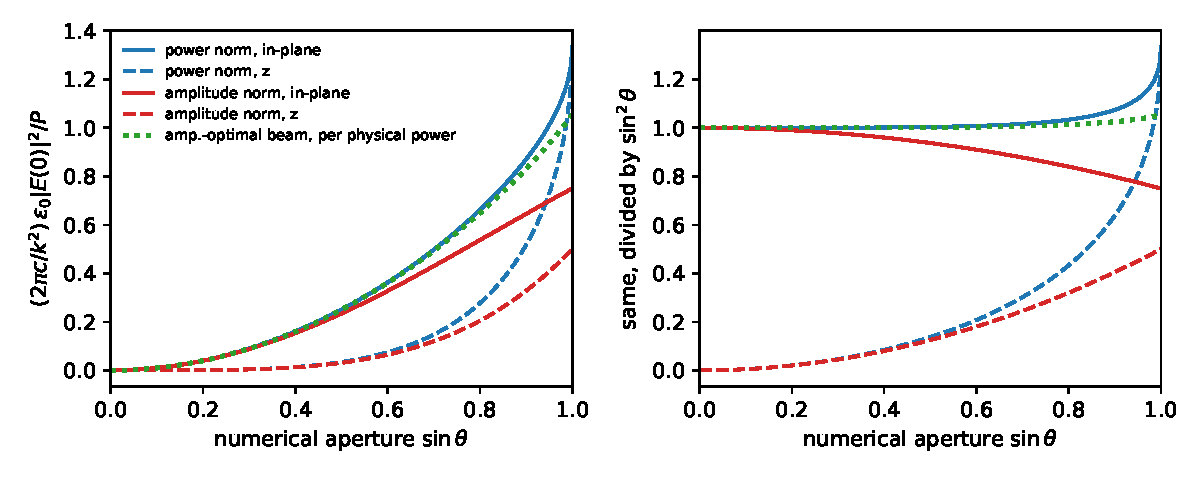
\includegraphics[width=0.85\linewidth]{focal_intensity_bounds.pdf}
\caption{Maximum focal intensity versus numerical aperture, \eqref{eq:bounds}. The dotted curve is the amplitude-optimal beam measured per unit physical power, \eqref{eq:ampTrue}.}
\label{fig:bounds}
\end{figure}

%=============================================================================
\section{The optimal fields across the focal plane}
%=============================================================================
\subsection{General numerical aperture}
Take $\qhat=\xhat$, write $\khat=(\sin\theta'\cos\varphi',\sin\theta'\sin\varphi',\cos\theta')$ and let the field point be at cylindrical coordinates $(\rho,\phi,z)$, with $a=k\rho$. The Cartesian components of $(\II-\khat\khat^{\rm T})\xhat$ are
\begin{align*}
\big(1-\sin^2\theta'\cos^2\varphi',\ -\tfrac12\sin^2\theta'\sin2\varphi',\ -\sin\theta'\cos\theta'\cos\varphi'\big).
\end{align*}
Shifting $\varphi'\to\varphi'+\phi$ in \eqref{eq:JA} gives
\begin{align}
\int {\rm d}\varphi'\,e^{iu\cos(\varphi'-\phi)}\{1,\ \cos^2\varphi'\} &= \{2\pi J_0(u),\ \pi[J_0(u)-\cos2\phi\,J_2(u)]\},\nonumber\\
\int {\rm d}\varphi'\,e^{iu\cos(\varphi'-\phi)}\{\sin2\varphi',\ \cos\varphi'\} &= \{-2\pi\sin2\phi\,J_2(u),\ 2\pi i\cos\phi\,J_1(u)\},
\end{align}
with $u=a\sin\theta'$. Hence, with $w(\theta')=1$ (power) or $|\cos\theta'|$ (amplitude normalization),
\begin{align}
    E_x &= \pi k^2\!\int\!{\rm d}\theta'\,\sin\theta'\,w\,e^{ikz\cos\theta'}\Big[(2-\sin^2\theta')J_0(u)+\sin^2\theta'\cos2\phi\,J_2(u)\Big],\nonumber\\
    E_y &= \pi k^2\sin2\phi\!\int\!{\rm d}\theta'\,\sin^3\theta'\,w\,e^{ikz\cos\theta'}J_2(u), \label{eq:fields1D}\\
    E_z &= -2\pi i k^2\cos\phi\!\int\!{\rm d}\theta'\,\sin^2\theta'\cos\theta'\,w\,e^{ikz\cos\theta'}J_1(u), \nonumber
\end{align}
with $\theta'\in[0,\theta]$ for one-sided excitation, and in addition $\theta'\in[\pi-\theta,\pi]$ for two-sided excitation. The focal spot is \emph{not} rotationally symmetric: $E_x$ depends on $\cos2\phi$, and $E_y\propto\sin2\phi$ and $E_z\propto\cos\phi$ both vanish on the axes. In particular $E_z$ is antisymmetric in $x$, with two lobes of opposite sign on either side of the focus along the polarization axis.
\numcheck{\code{focal\_plane\_fields.py}: \eqref{eq:fields1D} vs.\ brute-force 2D quadrature with explicit polarization vectors, rel.\ error $2\times10^{-14}$}

\subsection{Closed forms at \texorpdfstring{$2\pi$}{2 pi} solid angle}
For the power-optimal beam at $\theta=\pi/2$ and $z=0$, substitute $\beta=\sin\theta'$, so that $\sin\theta'{\rm d}\theta'=\beta\,{\rm d}\beta/\sqrt{1-\beta^2}$. The integrals reduce to the cases \eqref{eq:SonineCases}, together with
\begin{align*}
\int_0^1\frac{\beta^3J_0(a\beta)}{\sqrt{1-\beta^2}}{\rm d}\beta=j_0(a)-\int_0^1\beta\sqrt{1-\beta^2}J_0(a\beta){\rm d}\beta=j_0(a)-\frac{j_1(a)}{a}.
\end{align*} With $j_2=3j_1/a-j_0$:
\begin{align}
E_x &= 2\pi k^2\Big[\sin^2\!\phi\; j_0(a)+(3\cos^2\!\phi-1)\frac{j_1(a)}{a}\Big],\nonumber\\
E_y &= 2\pi k^2\sin\phi\cos\phi\; j_2(a),\qquad
E_z = -2\pi i k^2\cos\phi\,\frac{J_2(a)}{a},
\label{eq:2pi}
\end{align}
with $E_x(0)=4\pi k^2/3$. Comparing with the full-sphere result \eqref{eq:ImG} below shows that the in-plane part of \eqref{eq:2pi} is \emph{exactly one half} of the $4\pi$-optimal field in the focal plane. This follows from symmetry: under $z\to-z$ the lower cap maps to the upper one, the in-plane components of $(\II-\khat\khat^{\rm T})\xhat$ are even in $\hat k_z$, and $E_z$ is odd. Adding the mirror hemisphere therefore doubles $\Ev_\parallel$ and cancels $E_z$ at $z=0$.
\numcheck{closed form vs.\ quadrature $1.6\times10^{-14}$; $|\Ev_\parallel^{2\pi}-\tfrac12\Ev_\parallel^{4\pi}|/|\Ev|<10^{-16}$}

Along the polarization axis ($\phi=0$) and perpendicular to it ($\phi=\pi/2$):
\begin{align}
    |\Ev|^2_{\phi=0} = 4\pi^2k^4\Big[4\Big(\frac{j_1(a)}{a}\Big)^2+\Big(\frac{J_2(a)}{a}\Big)^2\Big],\qquad
    |\Ev|^2_{\phi=\pi/2} = 4\pi^2k^4\big[j_0(a)-j_1(a)/a\big]^2.
    \label{eq:2picuts}
\end{align}
The first is the expression printed in the tutorial, which is therefore the cut along the polarization axis. The second has \emph{exactly the same shape} as the $4\pi$ profile in the plane perpendicular to the polarization (Sec.~\ref{sec:4pi}). The $2\pi$-optimal spot is elliptical: its width along the polarization axis exceeds the paraxial Airy width, while its width perpendicular to the polarization is already the $4\pi$ value (Table~\ref{tab:widths}).

\paragraph{Amplitude normalization, any NA.} The extra $\cos\theta'$ turns the integrals into elementary Bessel integrals ($s=\sin\theta$, Bessel arguments $as$):
\begin{align}
    E_x = \pi k^2\Big[(2s-s^3)\frac{J_1}{a}+2s^2\frac{J_2}{a^2}+\cos2\phi\,s^3\frac{J_3}{a}\Big],\qquad
    E_y = \pi k^2\sin2\phi\,s^3\frac{J_3}{a},
    \label{eq:ampfields}
\end{align}
and at $s=1$, $E_z=-2\pi ik^2\cos\phi\,j_2(a)/a$ [last case of \eqref{eq:SonineCases}]. At $\phi=0$ the recurrences reduce $E_x$ to $\pi k^2s^2[(1-\tfrac{s^2}4)J_0+J_2+\tfrac{s^2}4J_4]$.
\numcheck{\code{tests/test\_sec3\_1.py}: rel.\ error $<5\times10^{-14}$ at $s=0.3,0.8,1$}

\paragraph{Paraxial limit.} For $\theta\ll1$ both normalizations give the Airy pattern,
\begin{align*}
E_x\simeq\int_{|\kp|\le k\sin\theta}\dkk\,e^{i\kp\cdot\xp}=2\pi k^2\sin^2\theta\,\frac{J_1(a\sin\theta)}{a\sin\theta},\qquad E_y,E_z\to0.
\end{align*}

\begin{figure}[tb]
\centering
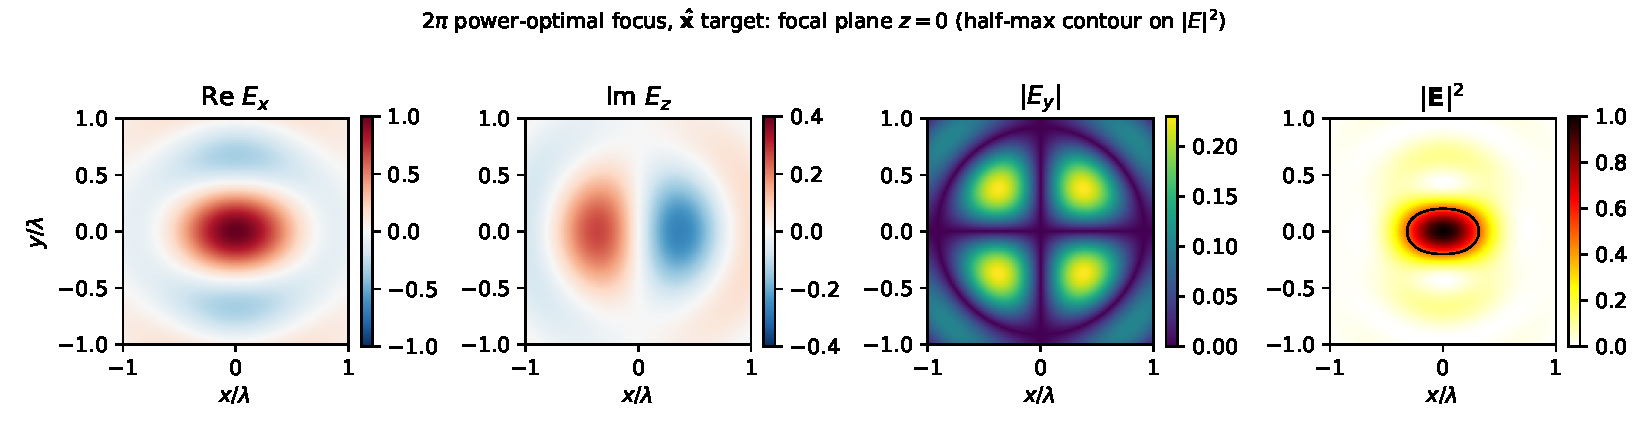
\includegraphics[width=\linewidth]{focal_plane_maps_2pi.pdf}\\[4pt]
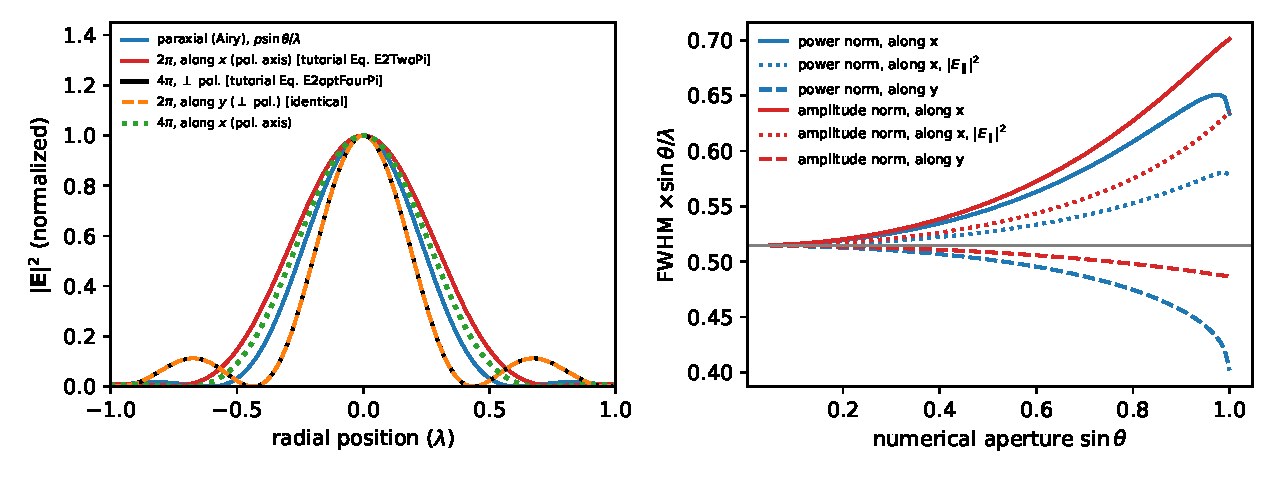
\includegraphics[width=0.95\linewidth]{focal_plane_profiles.pdf}
\caption{Top: focal-plane fields of the $2\pi$ power-optimal beam, \eqref{eq:2pi}. $E_z\propto\cos\phi$ is antisymmetric in $x$, and the half-maximum contour of $|\Ev|^2$ is an ellipse elongated along the polarization. Bottom left: intensity cuts. The $2\pi$ profile perpendicular to the polarization (dashed orange) coincides with the $4\pi$ profile (black). Bottom right: FWHM versus NA along the polarization axis ($x$, solid) and perpendicular to it ($y$, dashed); dotted curves show the in-plane intensity $|\Ev_\parallel|^2$ along $x$.}
\label{fig:fields}
\end{figure}

\begin{table}[tb]
\centering
\caption{Full widths at half maximum of $|\Ev|^2$ and locations of the first minimum, in wavelengths (paraxial row in units of $\lambda/\sin\theta$). ``First min.'' is a true zero only where $I/I_0\approx0$. The $4\pi$ beam is isotropic in the plane perpendicular to its polarization, so its $y$ and $z$ rows coincide.}
\label{tab:widths}
\begin{tabular}{llccc}
\toprule
excitation & direction & FWHM & first min. & $I/I_0$ there\\
\midrule
paraxial (Airy) & any & 0.5145 & 0.6098 & 0\\
$2\pi$, power norm. & $x$ (polarization) & 0.6337 & 0.7650 & $2.8\times10^{-3}$\\
 & $y$ & 0.4021 & 0.4367 & 0\\
 & $z$ (optical axis) & 0.8867 & 0.9898 & $1.6\times10^{-2}$\\
$2\pi$, amplitude norm. & $x$ & 0.7011 & 0.8734 & $1.4\times10^{-3}$\\
 & $y$ & 0.4865 & 0.5600 & 0\\
 & $z$ & 1.1862 & -- & --\\
$4\pi$ (power norm.) & $x$ (polarization) & 0.5777 & 0.7151 & 0\\
 & $y$, $z$ & 0.4021 & 0.4367 & 0\\
\bottomrule
\end{tabular}
\end{table}

Two features of Table~\ref{tab:widths} and Fig.~\ref{fig:fields} deserve emphasis:
\begin{enumerate}
\item In normalized units ($\rho\sin\theta/\lambda$), increasing the NA \emph{broadens} the spot along the polarization axis, from 0.51 to 0.63, but \emph{narrows} it perpendicular to the polarization, from 0.51 to 0.40. The width along $x$ is non-monotonic very close to $2\pi$ (maximum 0.651 near $\sin\theta\approx0.975$); this is a real feature of the optimal field, not a numerical artifact.
\item Relative to $2\pi$, the $4\pi$ optimum is tighter in the focal plane only along the polarization axis, because the lower hemisphere cancels $E_z$ (0.634 to 0.578). The large gain is along the optical axis (0.887 to 0.402). Perpendicular to the polarization the two profiles are identical.
\end{enumerate}

%=============================================================================
\section{Full \texorpdfstring{$4\pi$}{4 pi} solid angle (tutorial Sec.~3.1.3)}\label{sec:4pi}
%=============================================================================
\subsection{Herglotz form and the imaginary part of the Green's function}
For the full sphere, \eqref{eq:Herglotz} can be evaluated in closed form from
\begin{align*}
\int\dO\,e^{ik\khat\cdot\xv}=4\pi j_0(kr),\qquad \int\dO\,\hat k_i\hat k_je^{ik\khat\cdot\xv}=-k^{-2}\partial_i\partial_j[4\pi j_0(kr)].
\end{align*}
Using $j_0'=-j_1$ and $j_1'=j_0-2j_1/x$ ($x=kr$):
\begin{align}
    k^2\!\int\dO\,\big(\II-\khat\khat^{\rm T}\big)e^{ik\khat\cdot\xv}
    = 4\pi k^2\Big[\Big(j_0-\frac{j_1}{x}\Big)\II+\Big(\frac{3j_1}{x}-j_0\Big)\rhat\rhat^{\rm T}\Big]
    = 16\pi^2k\,\Im\mathsf{G}_0(\xv,0),
    \label{eq:ImG}
\end{align}
where $\mathsf G_0=(\II+\nabla\nabla/k^2)e^{ikr}/(4\pi r)$ is the free-space dyadic Green's function.
\numcheck{\code{fourpi\_spherical\_waves.py}: $8\times10^{-15}$}
The $4\pi$-optimal field is thus $\Im\mathsf G_0$ (the time-reversal field of Sec.~\ref{sec:TR}), and the $2\pi$-optimal field is ``half of $\Im\mathsf G_0$'', restricted to one hemisphere of directions. In the plane perpendicular to $\qhat$ ($\rhat\cdot\qhat=0$) the field is $4\pi k^2(j_0-j_1/x)\qhat$, isotropic in that plane. Along $\qhat$ it is $8\pi k^2(j_1/x)\qhat$.

\subsection{Vector spherical waves}
Define normalized vector spherical waves $\Mv_{\ell m}=z_\ell(kr)\vect X_{\ell m}$ and $\Nv_{\ell m}=k^{-1}\nabla\times\Mv_{\ell m}$, with $\vect X_{\ell m}=\vect L Y_{\ell m}/\sqrt{\ell(\ell+1)}$. Explicitly,
\begin{align}
    \Nv_{\ell m} = i\left[\sqrt{\ell(\ell+1)}\,\frac{z_\ell(x)}{x}Y_{\ell m}\rhat+\frac{1}{\sqrt{\ell(\ell+1)}}\,\frac{1}{x}\frac{{\rm d}[xz_\ell(x)]}{{\rm d}x}\nabla_sY_{\ell m}\right],
\end{align}
with $\nabla_s=\hat{\bm\theta}\partial_\theta+\hat{\bm\phi}\sin^{-1}\!\theta\,\partial_\phi$ and $z_\ell\in\{j_\ell,h^{(1)}_\ell,h^{(2)}_\ell\}$.
\numcheck{finite-difference $\nabla\times\Mv$ vs.\ $k\Nv$: $2\times10^{-10}$}
For regular waves at $r\to0$: $\Mv_{\ell m}\propto j_\ell\to0$; the radial part of $\Nv_{\ell m}$ is $\propto j_\ell(x)/x$, and the tangential part $\propto x^{-1}{\rm d}(xj_\ell)/{\rm d}x\to(\ell+1)x^{\ell-1}/(2\ell+1)!!$. Both vanish unless $\ell=1$. At the origin only the three electric-dipole waves survive, and
\begin{align}
    \Nv_{1,0}(0) = i\,\tfrac{1}{\sqrt2}\,\tfrac23\sqrt{\tfrac{3}{4\pi}}\,(\cos\theta\,\rhat-\sin\theta\,\hat{\bm\theta}) = i\,\tfrac23\sqrt{\tfrac{3}{8\pi}}\;\zhat,
\end{align}
and similarly for $m=\pm1$ along the spherical basis vectors.
\numcheck{scan of all regular VSWs with $\ell\le6$: only $(1,m)$ nonzero; $|\Nv_{1m}(0)|=0.2303294330$ exactly}
In the equatorial plane, ${\rm d}(xj_1)/{\rm d}x=xj_0-j_1$ gives $\Nv_{1,0}=-i\sqrt{3/(8\pi)}\,(j_0-j_1/x)\,\hat{\bm\theta}$, which is the tutorial's equatorial expression up to the overall phase convention.

\paragraph{Incoming power and the $4\pi$ bound.} The regular wave splits as $\Nv^{\rm reg}=\tfrac12(\Nv^{(1)}+\Nv^{(2)})$. In the far field $h^{(2)}_\ell(x)\to i^{\ell+1}e^{-ix}/x$, $\Nv^{(2)}$ is transverse with $\int|\Nv^{(2)}|^2r^2\dO\to k^{-2}\int|\nabla_sY|^2\dO/[\ell(\ell+1)]=k^{-2}$, and $|\Hv|=|\Ev|/Z_0$. Hence the incoming part $\tfrac12\Nv^{(2)}_{1,0}$ carries $P_{\rm in}=\tfrac12\cdot\tfrac14\cdot\tfrac1{Z_0k^2}=1/(8Z_0k^2)$, and
\begin{align}
    \frac{U(\xv_0)}{P_{\rm in}}=\frac{\tfrac14\varepsilon_0\cdot\tfrac49\cdot\tfrac{3}{8\pi}}{1/(8Z_0k^2)}=\frac{k^2}{3\pi c}.
\end{align}
\numcheck{inward Poynting flux at $R=3,30,300$: 0.1250000000; $U/P_{\rm in}=0.1061032954=1/(3\pi)$}
The three channels $\Nv_{1,m}$ have mutually orthogonal values at the origin and orthogonal fluxes. For any target $\qhat$, \eqref{eq:CS} therefore gives $\max|\qhat^*\cdot\Ev(0)|^2/P_{\rm in}=\sum_m|\qhat^*\cdot\Nv_{1m}(0)|^2/P_1=|\Nv_{10}(0)|^2/P_1$, which is independent of $\qhat$.

\paragraph{Doubling, in the plane-wave picture.} For a Herglotz wave $\Ev=\int\dO\,\vect a(\khat)e^{ik\khat\cdot\xv}$, stationary phase gives $\Ev\sim(2\pi/ikr)[\vect a(\rhat)e^{ikr}-\vect a(-\rhat)e^{-ikr}]$ as $r\to\infty$, so $P_{\rm in}=(2\pi^2/Z_0k^2)\int|\vect a|^2\dO$. For a one-sided beam this equals the $z$-directed power \eqref{eq:Power}, by \eqref{eq:dOmega}. With $\vect a=k^2(\II-\khat\khat^{\rm T})\qhat$: $|\Ev(0)|^2=(8\pi k^2/3)^2$ and $P_{\rm in}=(2\pi^2/Z_0)(8\pi/3)k^2$ for the full sphere, so $(2\pi c/k^2)\varepsilon_0|\Ev(0)|^2/P_{\rm in}=8/3$. Each hemisphere alone carries half the power and half the field, giving the $2\pi$ value $4/3$. The full-sphere Herglotz wave is proportional to $\Nv_{1,0}^{\rm reg}$ (ratio constant to $5\times10^{-12}$), and its incoming power computed from the VSW coefficient agrees with the stationary-phase value, $16\pi^3/3$, to all printed digits.

%=============================================================================
\section{Super-oscillatory spots (tutorial Sec.~3.1.4)}
%=============================================================================
\subsection{Minimum energy under point constraints}
For $E(x)=\int_{-k_m}^{k_m}c(k)e^{ikx}{\rm d}k$ the field energy is $\int|E|^2{\rm d}x=2\pi\int|c|^2{\rm d}k$. Minimizing $\int|c|^2$ subject to $E(x_i)=b_i$ is a minimum-norm problem, with solution $c(k)=\sum_i\lambda_ie^{-ikx_i}$ and
\begin{align}
    \min\int|c|^2{\rm d}k = \vect b^\dagger\mathsf{G}^{-1}\vect b,\qquad \mathsf{G}_{ij}=\int_{-k_m}^{k_m}e^{ik(x_i-x_j)}{\rm d}k=\frac{2\sin k_m(x_i-x_j)}{x_i-x_j}.
\end{align}
\paragraph{Two points.} The single constraint $E(x+\delta)-E(x)=1$ gives $\min\int|c|^2=1/\int|e^{ik\delta}-1|^2{\rm d}k=\big[4k_m-4\sin(k_m\delta)/\delta\big]^{-1}\to3/(2k_m^3\delta^2)$. This is the tutorial's $E\gtrsim1/\delta^2$, with its constant.

\paragraph{Three points.} Imposing $E(0)=1$ and $E(\pm\delta)=0$, the optimum is even in $k$ and the constraints are equivalent to $\int c=1$ and $\int c\,(1-\cos k\delta)=1$. The Gram matrix of $\{1,1-\cos k\delta\}$ has entries $2k_m$, $k_m^3\delta^2/3+O(\delta^4)$ and $k_m^5\delta^4/10+O(\delta^6)$, so
\begin{align}
    \min\int|c|^2{\rm d}k\ \to\ \frac{2k_m}{2k_m\cdot k_m^5\delta^4/10-k_m^6\delta^4/9}=\frac{45}{2k_m^5\delta^4},
    \qquad\frac{\text{constrained}}{\text{unconstrained}}\to\frac{45}{(k_m\delta)^4}.
\end{align}
The unconstrained optimum ($c$ uniform, energy $1/2k_m$) is the sinc beam, whose first zero is at $k_m\delta=\pi$, where the penalty is exactly 1. Halving the spot ($k_m\delta=\pi/2$) costs a factor of 5.28. The asymptotic formula overestimates this, predicting 7.4.
\numcheck{\code{superoscillation.py}: exact vs.\ asymptote ratio 0.9998 at $k_m\delta=0.03$}

\subsection{Zero ring in two dimensions}
In the paraxial scalar model with a circular pupil $|\kp|\le k_m$, a zero ring at radius $G$ constrains every angular harmonic of the pupil function. The focal amplitude involves only the $m=0$ harmonic, so the optimum sets the others to zero, leaving the single constraint $\int c_0(k)J_0(kG)k\,{\rm d}k=0$. Projecting the uniform pupil orthogonally to $J_0(kG)$ with the inner product $2\pi\int_0^{k_m}\!\cdot\,k\,{\rm d}k$, and using $\int_0^{k_m}J_0(kG)k\,{\rm d}k=k_mJ_1(u)/G$ and $\int_0^{k_m}J_0^2(kG)k\,{\rm d}k=\tfrac{k_m^2}{2}[J_0^2(u)+J_1^2(u)]$ with $u=k_mG$, the maximal Strehl ratio is
\begin{align}
    S_{\max}(u)=1-\frac{4J_1^2(u)}{u^2\big[J_0^2(u)+J_1^2(u)\big]}\ \xrightarrow{\ u\to0\ }\ \frac{u^4}{192},
\end{align}
with $S_{\max}=1$ at the Airy zero $u=3.8317$. The expansion follows from $[2J_1(u)/u]^2=1-\tfrac{u^2}4+\tfrac{5u^4}{192}$ and $J_0^2+J_1^2=1-\tfrac{u^2}4+\tfrac{6u^4}{192}$. In terms of the spot size normalized to the Airy zero, $S_{\max}\approx1.12\,(G/G_{\rm Airy})^4$. The exact penalties are $1/S_{\max}=9.3$ for a factor-of-2 reduction and $8.7\times10^3$ for a factor of 10. The naive $2^4=16$ therefore overstates the cost of a factor-of-2 reduction by about $1.7\times$; $S_{\max}(0.5)\approx0.1$ is also what the $S_{\max}$ curve of the tutorial's super-resolution figure shows.
\numcheck{closed form vs.\ brute-force pupil discretization: $<10^{-8}$}

\begin{figure}[tb]
\centering
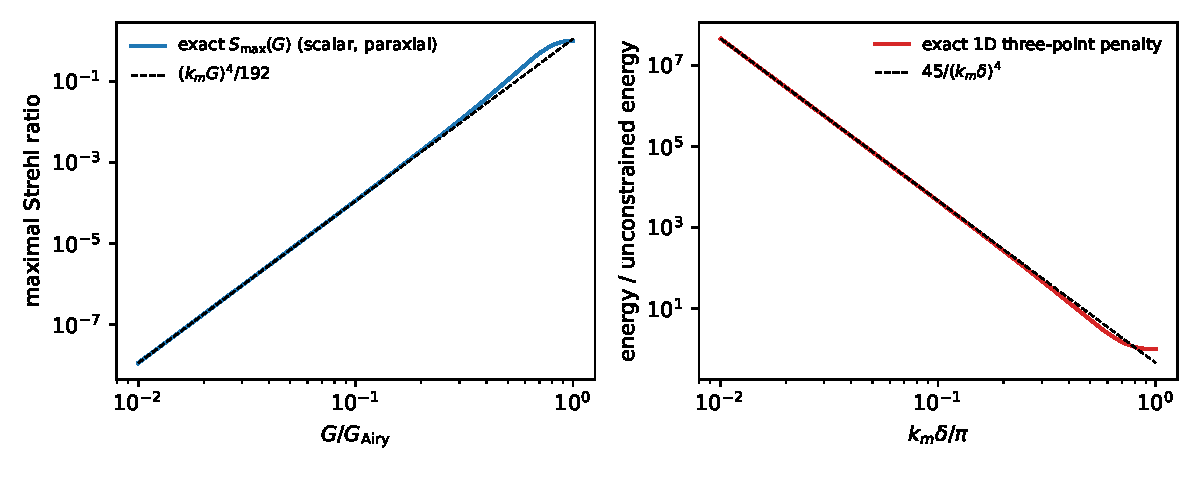
\includegraphics[width=0.8\linewidth]{superoscillation.pdf}
\caption{Left: exact maximal Strehl ratio for a zero ring (paraxial, scalar) and its $u^4/192$ asymptote. Right: exact 1D three-point energy penalty and its $45/(k_m\delta)^4$ asymptote.}
\end{figure}

%=============================================================================
\section{Space-time focusing (tutorial Sec.~3.1.5)}
%=============================================================================
Under amplitude normalization $\int\!\int|c(\kv,\omega)|^2=1$, \eqref{eq:CS} makes the optimal $c$ uniform on the support. For the 1D line (transverse wavenumber $|k|\le|\omega|/c$, $|\omega|\le\omega_m$):
\begin{align}
    \psi(x,t)&=\int_{-\omega_m}^{\omega_m}\!{\rm d}\omega\,\frac{2\sin(|\omega|x/c)}{x}e^{-i\omega t}
    =\frac{2}{x}\int_0^{\omega_m}\!\Big[\sin\omega\Big(\frac xc+t\Big)+\sin\omega\Big(\frac xc-t\Big)\Big]{\rm d}\omega\nonumber\\
    &=\frac{4c}{x}\Big[\frac{\sin^2(\omega_m(x+ct)/2c)}{x+ct}+\frac{\sin^2(\omega_m(x-ct)/2c)}{x-ct}\Big],
\end{align}
which is the tutorial's result. At $t=0$ it is $\propto\sin^2(\omega_mx/2c)/x^2$, with first zero at $2\pi c/\omega_m$, twice that of $\sin(\omega_mx/c)/x$.
\numcheck{\code{spacetime\_focusing.py}: vs.\ direct $(\omega,k)$ quadrature, $1.5\times10^{-14}$}

\paragraph{Three dimensions.} With uniform weight in $\omega$, the $t=0$ radial profile is $\int_0^{\omega_m}[j_0-j_1/u]_{u=\omega\rho/c}{\rm d}\omega=(c/\rho)\int_0^U(j_0-j_1/u){\rm d}u$ with $U=\omega_m\rho/c$. Using $\int_0^U j_1(u)/u\,{\rm d}u=\tfrac12[\Si(U)+\cos U/U-\sin U/U^2]$:
\begin{align}
    \psi_{\rm 3D}(\rho,0)\propto\frac{\Si(U)+j_1(U)}{U}=\frac43\Big[1-\frac{U^2}{15}+\dots\Big]\quad(U\to0),\qquad \to\frac{\pi}{2U}\quad(U\to\infty).
\end{align}
Because $\Si(U)>|j_1(U)|$ for all $U>0$, this profile has \emph{no zeros} and a non-oscillatory $1/\rho$ tail. Its intensity half width at half maximum is $1.80\times$ that of the single-frequency profile $j_0-j_1/U$. The 1D features (faster side-lobe decay, first zero doubled) are therefore specific to the 1D line.
\numcheck{closed form vs.\ quadrature $10^{-14}$; minimum over $0<U\le200$ is $+5.9\times10^{-3}$}

\paragraph{Dependence on the normalization.} Physical energy normalization changes the optimal weights. On the 2D line the per-frequency cost is $\int(k_z/k)|c|^2{\rm d}k_x$, so $c\propto k/k_z$ and the $t=0$ profile becomes $\int_0^{\omega_m}\omega J_0(\omega x/c){\rm d}\omega\propto J_1(U)/U$ (versus single-frequency $J_0(U)$; first-zero ratio 1.593). In 3D the incoming energy of a Herglotz pulse is $\propto\int{\rm d}\omega\int\dO|\vect a|^2/\omega^2$, so $\vect a\propto\omega^2$ and the profile is $\propto[2\sin U-U\cos U-\Si(U)]/U^3$, which does have zeros (first at $U=3.797$, versus 2.744 for a single frequency). The qualitative conclusion, that temporal localization costs spatial localization, survives. The factor of 2 and the side-lobe behavior do not.

\begin{figure}[tb]
\centering
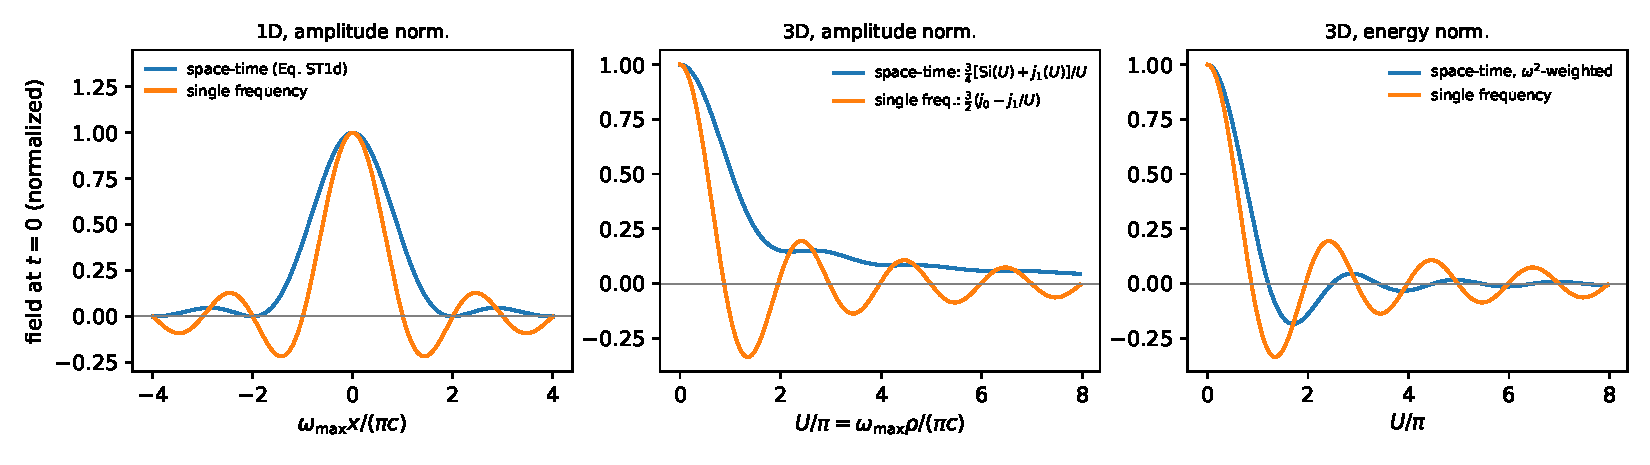
\includegraphics[width=\linewidth]{spacetime_focusing.pdf}
\caption{$t=0$ profiles of space-time-optimal fields (blue) versus single-frequency optima at $\omega_{\max}$ (orange), for the 1D line and 3D, and in 3D for energy normalization.}
\end{figure}

%=============================================================================
\section{Focusing in complex media (tutorial Sec.~3.2)}
%=============================================================================
\subsection{The bound and the optimal currents}
Currents $s$ on an aperture $A$ produce $\psi(\xv_0)=\Gamma_{0A}s$. For a target polarization $\phi$, the objective $|\phi^\dagger\Gamma_{0A}s|^2$ with $\|s\|=1$ is rank one, so by \eqref{eq:CS}
\begin{align}
    \max|\phi^\dagger\psi(\xv_0)|^2=\|\Gamma_{0A}^\dagger\phi\|^2=\int_A\big|(\Gamma_{0A}^\dagger\phi)(\xv')\big|^2{\rm d}\xv',\qquad s_{\rm opt}\propto\Gamma_{0A}^\dagger\phi.
\end{align}
Nothing about the medium has been assumed. If the medium is reciprocal, $\Gamma(\xv_0,\xv')^{\rm T}=\Gamma(\xv',\xv_0)$, then $(\Gamma_{0A}^\dagger\phi)(\xv')=[\Gamma(\xv',\xv_0)\phi^*]^*$, the conjugate of the field on $A$ radiated by a dipole $\phi^*$ at $\xv_0$. If the medium is not reciprocal, generalized reciprocity $\Gamma_\nu(\xv,\xv')^{\rm T}=\Gamma_{\nu^{\rm T}}(\xv',\xv)$ gives the same recipe in the \emph{transposed} medium.

\paragraph{Far-field aperture and the LDOS.} For a closed aperture in the far zone of a lossless medium, $|\Ev|=Z_0|\Hv|$ and $\int_A|\Ev_0|^2{\rm d}A=2Z_0P_{\rm rad}$, where $P_{\rm rad}=\tfrac\omega2\Im(\pv^*\cdot\Ev(\xv_0))$ is the power radiated by the dipole, i.e.\ the LDOS. For apertures in the near field the bound is larger.

\subsection{A point-dipole medium with controllable symmetries}\label{sec:dipole-medium}
To test these statements we use electric point scatterers $\pv_j=\alpha_j\Ev_{\rm loc}(\xv_j)$ with $\alpha_j^{-1}=\alpha_{0,j}^{-1}-i\tfrac{k^3}{6\pi\varepsilon_0}\II$, where the radiation-reaction term is $\varepsilon_0^{-1}k^2\Im\mathsf G_0(0)$. With $\Ev=\varepsilon_0^{-1}k^2\mathsf G_0\pv$, the medium Green's function is
\begin{align}
    \Gamma(\xv,\xv')=\frac{k^2}{\varepsilon_0}\Big[\mathsf G_0(\xv,\xv')+\frac{k^2}{\varepsilon_0}\mathsf G_0(\xv,S)\,\mathsf T\,\mathsf G_0(S,\xv')\Big],\qquad \mathsf T=\big(\operatorname{diag}\alpha_j^{-1}-\tfrac{k^2}{\varepsilon_0}\mathsf G_{SS}\big)^{-1},
\end{align}
where $\mathsf G_{SS}$ couples distinct scatterers. All blocks of $\mathsf G_0$ are symmetric and $\mathsf G_0(\xv,\xv')=\mathsf G_0(\xv',\xv)$, so $\mathsf T^{\rm T}=\mathsf T|_{\alpha\to\alpha^{\rm T}}$. The symmetries of the medium are then controlled entirely by $\alpha_0$:
\begin{itemize}
\item \emph{reciprocal} $\Leftrightarrow\alpha_0^{\rm T}=\alpha_0$. In general, $\Gamma_{\alpha}(\xv,\xv')^{\rm T}=\Gamma_{\alpha^{\rm T}}(\xv',\xv)$.
\item \emph{lossless} $\Leftrightarrow\alpha_0^\dagger=\alpha_0$. The power absorbed by dipole $j$ is $\tfrac\omega2\pv^\dagger\big[(\alpha_0^{-1})^\dagger-\alpha_0^{-1}\big]\pv/(2i)$, the radiation-reaction term accounting exactly for the scattered power $\tfrac{\omega k^3}{12\pi\varepsilon_0}|\pv|^2$.
\item \emph{time-reversal invariant} $\Leftrightarrow\alpha_0$ real. Under $(\Ev,\Hv,\pv,\mv)\to(\Ev^*,-\Hv^*,\pv^*,-\mv^*)$ the constitutive relation $\pv=\alpha_0\Ev_{\rm loc}$ maps to itself iff $\alpha_0^*=\alpha_0$. The radiation-reaction term is part of the outgoing boundary condition, not of the medium.
\end{itemize}
The four test media are lossless reciprocal ($\alpha_0$ real symmetric), lossy reciprocal (complex symmetric), \emph{TRI but non-reciprocal} (real, non-symmetric), and gyrotropic (Hermitian, non-symmetric: lossless, non-reciprocal, non-TRI).

\subsection{Numerical results}
Table~\ref{tab:recipe} tests the bound and the recipes with random clusters of 16 scatterers in a $\lambda^3$ box, a random complex target polarization, and electric currents on either an open near-field patch or a closed sphere of radius $6\lambda$. $\Gamma$ is built directly from $\mathsf T$, without invoking reciprocity. The iterative eigen-solution of the full operator confirms the rank-one maximum in all cases (rel.\ difference $\le2\times10^{-15}$).

\begin{table}[tb]
\centering
\caption{Achieved focal intensity divided by the bound, for currents prescribed by the conjugated dipole field computed in the actual medium (``recipe'') or in the transposed medium (\code{complex\_media\_focusing.py}).}
\label{tab:recipe}
\begin{tabular}{lcccc}
\toprule
 & \multicolumn{2}{c}{open near-field patch} & \multicolumn{2}{c}{closed sphere, $R=6\lambda$}\\
medium & recipe & transposed & recipe & transposed\\
\midrule
lossless, reciprocal & 1.00000000 & 1.00000000 & 1.00000000 & 1.00000000\\
lossy, reciprocal & 1.00000000 & 1.00000000 & 1.00000000 & 1.00000000\\
TRI, non-reciprocal & 0.216 & 1.00000000 & 0.084 & 1.00000000\\
gyrotropic & 0.265 & 1.00000000 & 0.231 & 1.00000000\\
\bottomrule
\end{tabular}
\end{table}

For the LDOS connection, closed spheres about $\xv_0$ in the lossless reciprocal medium give bound$/(2P_{\rm rad})$ = 94.8, 45.8, 1.012 and 1.00012 for $R=0.06$, 0.3, 3 and $30\lambda$. The sphere with $R=0.3\lambda$ passes through the cluster, and any aperture is allowed.

\subsection{Partial time reversal on a closed surface}\label{sec:TR}
In the representation $\psi=(\Ev,i\Hv)$, $s=(i\Jv_e,-\Jv_m)$ of the tutorial, complex conjugation is time reversal: $\Ev\to\Ev^*$, $\Hv\to-\Hv^*$, $\Jv_e\to-\Jv_e^*$, $\Jv_m\to\Jv_m^*$ (for point dipoles, $\pv\to\pv^*$, $\mv\to-\mv^*$). The four-step construction of the tutorial proceeds as follows. The Love currents $\Jv_s=\nhat\times\Hv$, $\Jv_{m,s}=-\nhat\times\Ev$ on a closed surface $S$ enclosing all sources and scatterers radiate $(\Ev,\Hv)$ outside $S$ and zero inside, in the actual medium, since the scatterers inside $S$ see no field. Their negatives are the perfectly cancelling currents $s_{\rm pcc}$. If the medium is TRI, conjugation gives $M\psi^*=s_0^*+s_{\rm pcc}^*$, so
\begin{align}
    \psi_{\rm TR}\equiv\Gamma s_{\rm pcc}^*=\psi^*-\Gamma s_0^*=
    \begin{cases}-2i\Im\psi & \xv\text{ inside }S\ (s_0\text{ real}),\\ -\Gamma s_0^* & \xv\text{ outside }S.\end{cases}
\end{align}
The entrywise-$\Im\Gamma$ form of the tutorial therefore holds for field points inside $S$. Reciprocity was not used at any step.

The numerical test uses a real dipole inside a sphere $S$ of radius $\lambda$, with one scatterer placed $0.05\lambda$ from $S$ to test the claim that no far-field assumption is needed. Fields and Love currents are evaluated with a $180\times360$ Gauss--Legendre$\times$trapezoid quadrature on $S$. Time-reversed currents are radiated in the medium, and the result is compared with $-2i\Im\Ev$ at 25 interior points:
\begin{center}
\begin{tabular}{lcc}
\toprule
medium & $\max|\psi_{\rm TR}+2i\Im\Ev|/\max|2\Im\Ev|$ inside $S$ & extinction-theorem residual\\
\midrule
lossless, reciprocal (TRI) & $7\times10^{-8}$ & $2\times10^{-7}$\\
TRI, non-reciprocal & $1\times10^{-6}$ & $4\times10^{-6}$\\
lossy, reciprocal (not TRI) & 0.45 & $2\times10^{-7}$\\
gyrotropic (not TRI) & 1.24 & $1\times10^{-6}$\\
\bottomrule
\end{tabular}
\end{center}
The residuals of the TRI cases fall with quadrature refinement, tracking the extinction-theorem residual (at $120\times240$ they are $5\times10^{-6}$ and $6\times10^{-5}$). The failures are $O(1)$ and do not change. This supports two statements of the tutorial: that time reversal, not reciprocity, underlies the conjugate-field identity, and that the time-reversal recipe and the reciprocity recipe are distinct. In the TRI non-reciprocal medium the time-reversed field is exactly $-2i\Im\Ev$, yet the conjugate-field recipe reaches only 8--22\% of the maximum focal intensity (Table~\ref{tab:recipe}).

\subsection{Space-time version}
With sources $s(\xv,t)$ on $A$ for $t\in[0,T]$, $\psi(\xv_0,t_0)=\int_0^T{\rm d}t\int_A\Gamma_{\rm ret}(\xv_0,t_0;\xv,t)s(\xv,t)$, which is again rank one. By time-domain reciprocity and time-translation invariance, $\Gamma_{\rm ret}(\xv_0,t_0;\xv,t)^{\rm T}=\Gamma_{\rm ret}(\xv,t_0-t;\xv_0,0)$. The optimal source is then $s(\xv,t)\propto\psi_0(\xv,t_0-t)$: the field of a dipole fired at $(\xv_0,0)$, time-reversed. The bound is
\begin{align}
    \max|\phi^{\rm T}\psi(\xv_0,t_0)|^2=\int_{t_0-T}^{t_0}{\rm d}\tau\int_A|\psi_0(\xv,\tau)|^2{\rm d}\xv,
\end{align}
which reduces to the window $[0,T]$ written in the tutorial when the focal time is the end of the source window, $t_0=T$.

%=============================================================================
\section{Index of numerical checks}
%=============================================================================
\begin{center}
\small
\begin{tabular}{lll}
\toprule
result & script (repository) & agreement\\
\midrule
plane-wave power formula & \code{power\_normalization\_check.py} & $10^{-16}$\\
focal-intensity maxima, optimal polarization & \code{focal\_intensity\_bounds.py} & $3\times10^{-13}$\\
amplitude-optimal beam per physical power & \code{focal\_intensity\_bounds.py} & $10^{-14}$\\
focal-plane fields, closed forms, $\tfrac12$ of $4\pi$ & \code{focal\_plane\_fields.py} & $2\times10^{-14}$\\
widths (Table~\ref{tab:widths}) & \code{focal\_plane\_fields.py} & $10^{-4}$ (root finding)\\
VSW amplitudes, $P_{\rm in}$, $k^2/3\pi c$, $\Im\mathsf G_0$ & \code{fourpi\_spherical\_waves.py} & $10^{-10}$--$10^{-15}$\\
super-oscillation penalties, $S_{\max}$ & \code{superoscillation.py} & $10^{-8}$\\
space-time profiles & \code{spacetime\_focusing.py} & $10^{-14}$\\
complex-media bound, recipes, TR identity & \code{complex\_media\_focusing.py} & $10^{-15}$ / $10^{-7}$\\
\bottomrule
\end{tabular}
\end{center}
All scripts run in seconds on a laptop (Python 3 with NumPy, SciPy, Matplotlib); \code{pytest tests/} runs the regression versions.

\end{document}
